\subsection{Descriptive Statistics and Stylized Facts}
\label{sec:descriptive}

All three canonical stylized facts are present in both the IS ($T = 2{,}516$) and OoS ($T = 572$) windows.
The IS excess growth rates exhibit excess kurtosis of $7.678$, strong negative skewness ($-0.751$), and a Jarque--Bera statistic of $6{,}416.6$, decisively rejecting normality ($p < 0.001$).
The Ljung--Box test on absolute returns rejects no autocorrelation ($\text{LB} = 2{,}959.3$, $p < 0.001$), confirming pronounced volatility clustering.
The OoS window shares the same qualitative profile (excess kurtosis $5.294$, $\text{LB}_{|G|} = 250.6$).

\subsection{State-Count Selection}
\label{sec:k_selection_results}

We sweep $K \in \{3, 6, 9, 12, 15, 18, 21\}$ for CHMM-N on the SPY IS window, scoring each fitted model on the four information criteria of \citet{nguyen2018hidden} (AIC, BIC, HQC, CAIC, with $p = K^2 + 2K - 1$ parameters) and on the IS / OoS Kolmogorov--Smirnov pass rate.
Two structural patterns emerge.
The information-criterion surface flattens over the upper half of the sweep: BIC and CAIC reach their joint minimum in the $K \in \{15, 18, 21\}$ region. Distributional fidelity rises across the sweep and plateaus in the same band: IS KS rises from $89.8\%$ ($K = 3$) to $94.7\%$ at $K = 18$. ACF-MAE, by contrast, is remarkably stable across the entire sweep ($0.047$--$0.053$), consistent with the spectral identity~\eqref{eq:acf_normalised}: the ACF is determined by the eigenvalue spectrum of $\mathbf T$, which the quantile-initialized Baum-Welch recovers at every $K \ge 3$.
We report the remainder of this section at the operating point $K = 18$, which sits inside the IC-minimizing band and at the top of the distributional plateau; results at $K = 3, 6, 9, 12, 15, 21$ are reported in Appendix~\ref{sec:supplementary}.

\subsection{Six-Generator Comparison (Pipeline~A)}
\label{sec:model_comparison}

This subsection operates under Pipeline~A (Figure~\ref{fig:pipeline_schematic}, top row): every generator is fit independently to the SPY return series, no cross-asset coupling. Table~\ref{tab:model_comparison} reports the IS and OoS validation results for the three benchmark generators of Section~\ref{sec:benchmarks} together with the three CHMM emission variants at $K = 18$.

\begin{table}[t]
\centering
\caption{\textbf{Six-generator comparison on SPY}. $K = 18$, $1{,}000$ simulated paths, $\alpha = 0.05$. IS: 2014-01-03 through 2024-01-03 ($T = 2{,}516$); OoS: 2024-01-04 through 2026-04-20 ($T = 572$). KS = Kolmogorov--Smirnov pass rate (\%); Kurt = mean simulated excess kurtosis (observed: $7.68$ IS, $5.29$ OoS); ACF-MAE = mean absolute error of $\text{ACF}(|G_t|)$ over $252$ lags.}
\label{tab:model_comparison}
\small
\begin{tabular}{l cc cc c}
\toprule
& \multicolumn{2}{c}{KS (\%) $\uparrow$} & \multicolumn{2}{c}{Kurtosis} & ACF-MAE \\
\cmidrule(lr){2-3} \cmidrule(lr){4-5}
Model & IS & OoS & IS & OoS & $\downarrow$ \\
\midrule
\textit{Observed}                    & --   & --   & $7.68$  & $5.29$  & --     \\
Bootstrap                            & $99.9$ & $91.0$ & $7.54$  & $6.80$  & $0.0628$ \\
Gaussian i.i.d.                      & $0.0$  & $1.2$  & $-0.01$ & $-0.02$ & $0.0627$ \\
Laplace i.i.d.                       & $99.1$ & $86.1$ & $2.96$  & $2.83$  & $0.0627$ \\
GARCH(1,1)                           & $25.9$ & $58.2$ & $6.97$  & $2.88$  & $0.0484$ \\
\textbf{CHMM-N ($K = 18$)}           & $93.8$ & $84.2$ & $4.99$  & $4.51$  & $\mathbf{0.0507}$ \\
\textbf{CHMM-t ($K = 18$)}           & $93.7$ & $85.9$ & $14.57$ & $9.74$  & $0.0548$ \\
\textbf{CHMM-L ($K = 18$)}           & $93.2$ & $79.3$ & $\mathbf{6.75}$  & $\mathbf{6.27}$  & $0.0565$ \\
\bottomrule
\end{tabular}
\end{table}

The headline finding is in the bottom three rows.
At $K = 18$, CHMM-N attains $93.8\%$ IS KS and $84.2\%$ OoS KS, comparable to the bootstrap distributional ceiling and substantially above GARCH ($25.9\%$ IS KS); ACF-MAE of $0.0507$ is essentially on par with GARCH ($0.0484$), the empirical instance of the spectral identity~\eqref{eq:acf_normalised}: with $K-1 = 17$ non-unit eigenvalues at the operating point, the mixture-of-eigenvalues sum reproduces the slow absolute-return ACF that the \citet{ryden1998stylized} $K = 2$--$3$ Gaussian setup could not recover, inside a standard HMM at moderate state resolution.
The bootstrap (at $0.0628$) and the i.i.d.\ baselines all sit far above the temporal floor.

The three CHMM emission variants land at three distinct points on the kurtosis axis without retuning $K$ or the transition structure: CHMM-N undershoots ($5.0$ IS vs.\ observed $7.7$), CHMM-t overshoots ($14.6$, an artefact discussed in Section~\ref{sec:discussion}), and CHMM-L matches cleanly ($6.8$, within $0.9$ units of observed). CHMM-L is the strongest entry on IS kurtosis in the panel and adds no shape parameter to CHMM-N (location is the weighted median, scale is the weighted mean absolute deviation, both in closed form). All three variants match each other on KS pass rates to within $1$ percentage point IS and within $7$ percentage points OoS, and all three are within $0.006$ of each other on ACF-MAE: the emission-family swap moves tail weight cleanly without disturbing the central or temporal fit.

GARCH wins on ACF-MAE alone but fails distributional KS decisively; the bootstrap wins KS but is the worst on ACF-MAE; the CHMM at moderate $K$ occupies a distinctive corner where both metrics simultaneously sit close to their respective best-in-panel values, and the choice between CHMM-N, CHMM-t, and CHMM-L is the choice of where to land the kurtosis residual.

\begin{figure}[t]
\centering
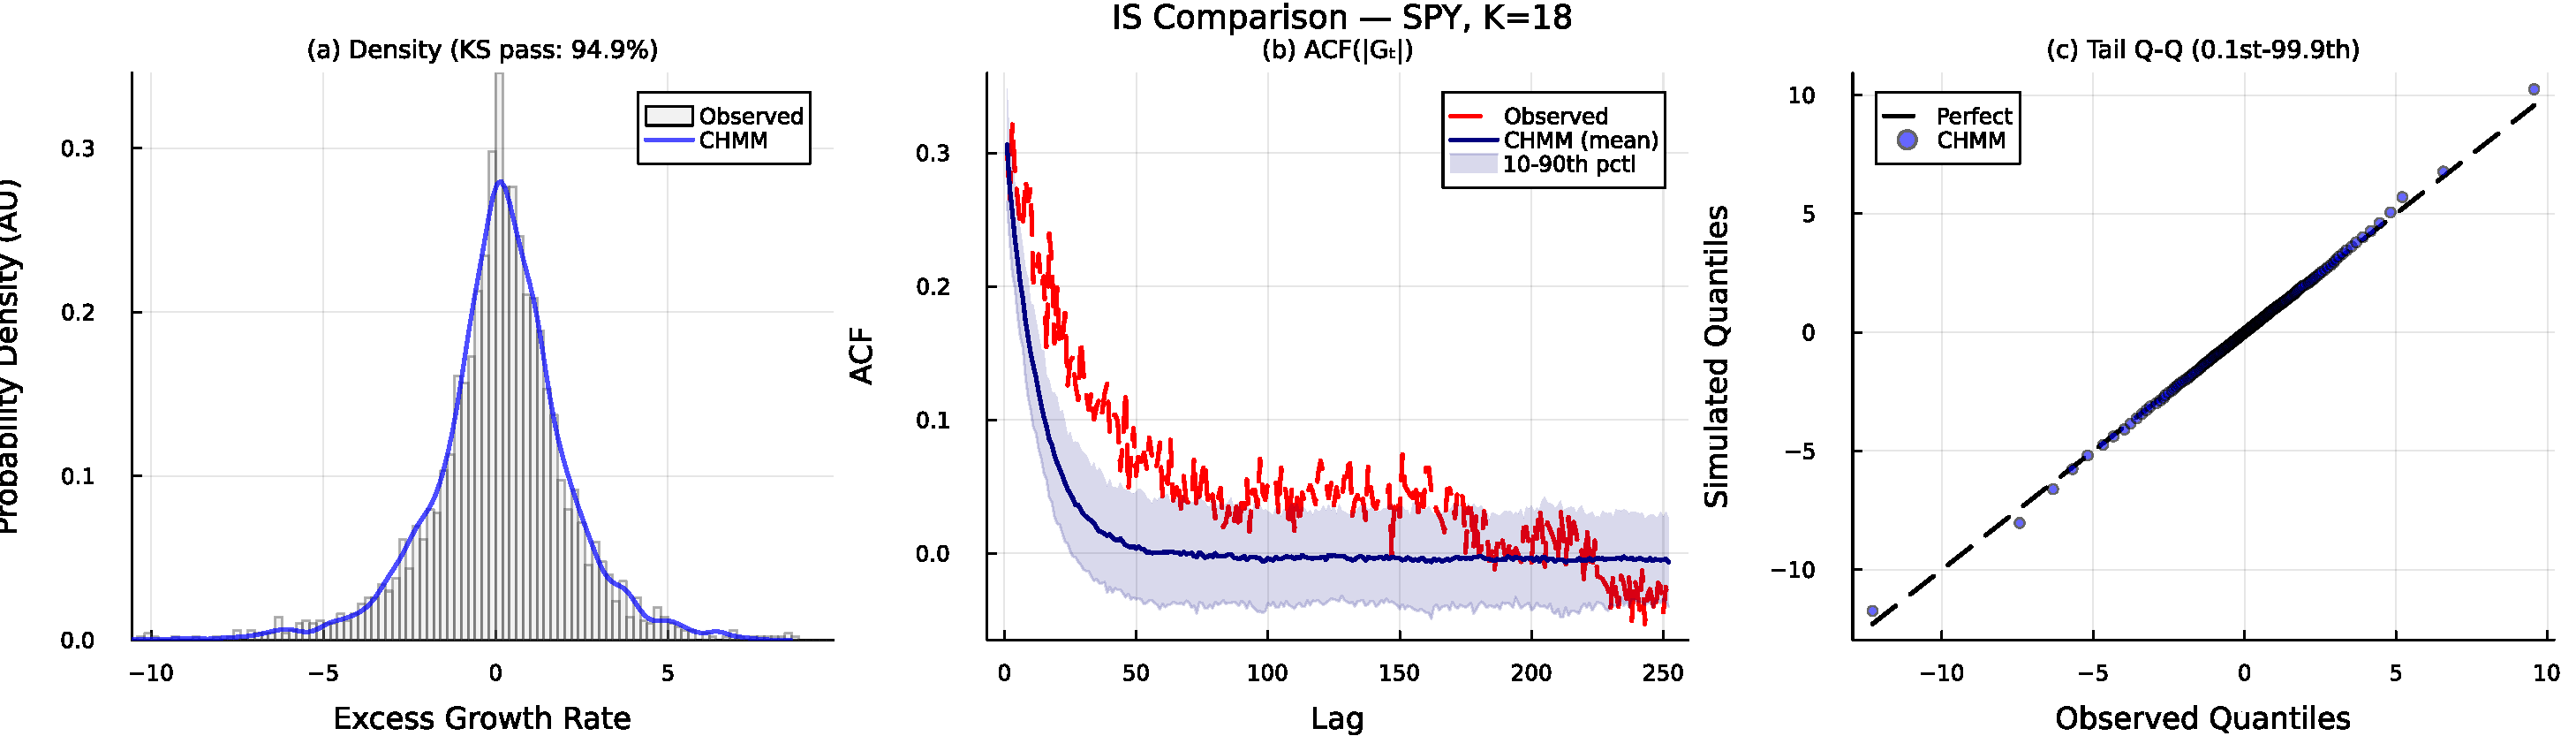
\includegraphics[width=\textwidth]{figs/Fig-3-IS-Comparison-K18.pdf}
\caption{\textbf{IS CHMM-N validation on SPY} ($K = 18$, $1{,}000$ simulated paths). Panel~(a): marginal density of the annualized excess log return $G_t$; gray histogram $=$ observed IS series, blue curve $=$ one simulated path. Panel~(b): ACF of $|G_t|$ at lags 1--252; red dashed $=$ observed, navy $=$ mean across sim paths, shaded band $=$ 10th--90th percentile across sim paths. Panel~(c): tail Q-Q plot at $200$ quantile levels; blue points $=$ simulated pooled over paths, black dashed $=$ identity.}
\label{fig:is_comparison}
\end{figure}

\subsection{Cross-Ticker Generalization (Pipeline~A)}
\label{sec:cross_asset_univariate}

Still under Pipeline~A: each ticker is fit independently, no cross-asset coupling.
Table~\ref{tab:cross_ticker} reports CHMM-t IS and OoS KS pass rates across the five additional tickers (NVDA, JNJ, JPM, AAPL, QQQ), each fit independently at $K = 18$. CHMM-t is the natural generalization vehicle here because it carries the strongest OoS KS in the SPY headline panel ($85.9\%$, against $84.2\%$ for CHMM-N and $79.3\%$ for CHMM-L) and supplies the per-state heavy tails that the outlier-prone single-name tickers (NVDA, JNJ) require. Per-family $K$-sensitivity for SPY across all three emission variants and per-ticker price-level metrics across all three families are in Appendix~\ref{sec:supplementary}.
The univariate fidelity persists across the panel on IS KS ($95.2\%$ to $99.8\%$). On OoS, JNJ, AAPL, and QQQ generalise cleanly ($90$--$95\%$), while NVDA ($57.2\%$) and JPM ($53.0\%$) show substantial OoS degradation, a stationarity artefact: the IS-fixed transitions and emissions cannot capture the AI-driven NVDA regime or the rate-repricing cycle for financials in the $2024$--$2026$ holdout.
A walk-forward quarterly refit recovers $\sim 15$ percentage points of the JPM gap (Appendix~\ref{sec:supplementary}); we acknowledge the residual cliff as a stationarity-scope limitation rather than a model-selection issue (it persists at every $K$ in the sweep).

\begin{table}[t]
\centering
\caption{\textbf{Cross-ticker generalization, CHMM-t at $K = 18$}. Each ticker fit independently; $1{,}000$ simulated paths, $\alpha = 0.05$. Observed kurtosis is the IS sample value.}
\label{tab:cross_ticker}
\small
\begin{tabular}{l cc c c c}
\toprule
& \multicolumn{2}{c}{KS (\%) $\uparrow$} & \multicolumn{2}{c}{Kurtosis} & ACF-MAE \\
\cmidrule(lr){2-3} \cmidrule(lr){4-5}
Ticker & IS & OoS & Obs & Sim & $\downarrow$ \\
\midrule
SPY  & $95.2$ & $84.1$ & $7.7$ & $14.68$ & $0.0551$ \\
NVDA & $99.1$ & $57.2$ & $5.5$ & $46.40$ & $0.0478$ \\
JNJ  & $99.8$ & $94.3$ & $9.0$ & $99.66$ & $0.0332$ \\
JPM  & $99.2$ & $53.0$ & $7.6$ & $18.82$ & $0.0483$ \\
AAPL & $99.1$ & $94.7$ & $3.2$ & $7.54$  & $0.0424$ \\
QQQ  & $96.1$ & $90.3$ & $3.4$ & $3.30$  & $0.0576$ \\
\bottomrule
\end{tabular}
\end{table}

\subsection{Rolling-Origin Out-of-Sample (Pipeline~A)}
\label{sec:rolling_origin}

Still under Pipeline~A: only the IS / OoS fit window rolls forward, no cross-asset coupling is introduced.
The single $2024$--$2026$ OoS window above is qualified by a five-window rolling-origin evaluation (eight-year IS, one-year OoS, sliding through $2022$--$2026$) at $\alpha = 0.05$ on the unconditional Kupiec test.
The $2022$ window is a structural counter-example: the rate-hike cycle is not represented in the preceding eight years of near-zero rates, OoS KS collapses to $0.2$--$0.4\%$, and Kupiec rejects with $\text{LR}_{\text{uc}}^{5\%} = 31.6$--$41.4$.
The $2024$, $2025$, and $2026$-year-to-date windows all pass Kupiec at $5\%$ cleanly with OoS KS in the $87$--$97\%$ range, and the $2023$ window is intermediate.
Excluding the $2022$ structural-break window, CHMM-t IS KS is $95.8\% \pm 1.6\%$ and OoS KS is $91.1\% \pm 3.5\%$.
The headline single-window result is closer to the modal behaviour than to the worst case, and the $2022$ window is the most informative single piece of negative evidence on the stationarity scope: the CHMM scaffold is well-calibrated when the IS window contains volatility regimes comparable to those of the OoS window, and fails predictably under structural breaks that lie outside the IS support. A rolling refit of $\hat{\mathbf{T}}$ and the emissions each quarter is the natural operational remedy.

\begin{figure}[t]
\centering
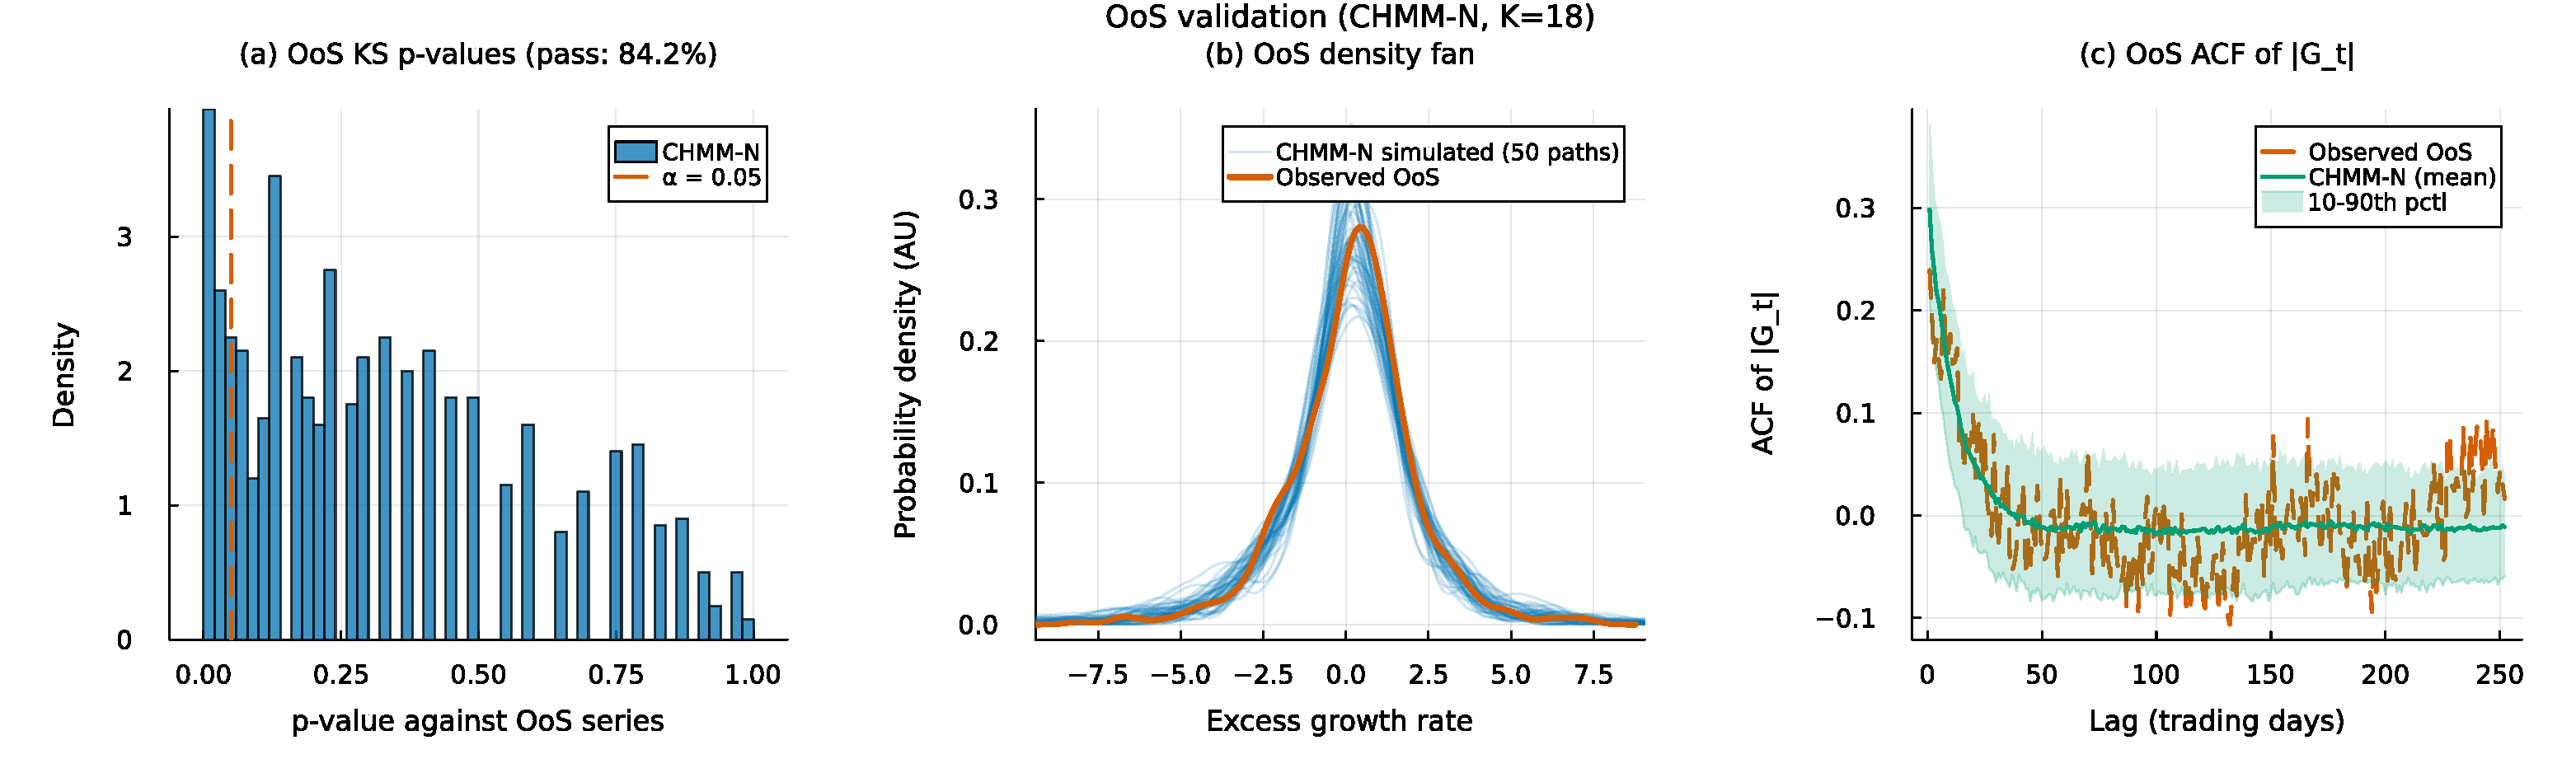
\includegraphics[width=\textwidth]{figs/Fig-4-OoS-Validation-K18.pdf}
\caption{\textbf{OoS CHMM-N validation on SPY} ($K = 18$, $1{,}000$ paths, $T_{\text{OoS}} = 572$). Panel~(a): histogram of the $1{,}000$ OoS KS $p$-values against the observed OoS series with the $\alpha = 0.05$ threshold (red dashed). Panel~(b): OoS return-density fan; blue thin curves $=$ simulated densities, red thick curve $=$ observed OoS density. Panel~(c): ACF of $|G_t|$ on the OoS window; red dashed $=$ observed, navy $=$ mean across sim paths, shaded band $=$ 10th--90th percentile.}
\label{fig:oos_validation}
\end{figure}

\subsection{Cross-Asset Dependence (Pipeline~B): Student-t Copula}
\label{sec:cross_asset}

This subsection is the only Pipeline~B subsection in the main text (Figure~\ref{fig:pipeline_schematic}, bottom row): we reuse the per-asset CHMM-N marginals from the Pipeline-A fits of Section~\ref{sec:cross_asset_univariate} and add a cross-asset dependence layer on top.
For multi-asset synthesis we inject cross-sectional dependence through the rank-based Student-t copula of Section~\ref{sec:cross_asset_methods}, the strongest dependence layer in our larger panel; the SIM and Gaussian copula constructions are reported in Appendix~\ref{sec:supplementary}.
The per-asset marginals here are the CHMM-N fits at $K = 18$; rank reordering preserves whichever marginal it receives exactly (Proposition~\ref{prop:rank_marginals}), so the dependence-layer ranking is invariant to the choice of CHMM emission family, and the Pipeline-B numbers below transfer unchanged to CHMM-t or CHMM-L marginals up to the per-asset KS sanity-check column.
Profile maximum likelihood over $\nu \in \{2, 3, 4, 5, 6, 8, 10, 15, 20, 30\}$ on the six-asset universe (SPY, NVDA, JNJ, JPM, AAPL, QQQ; $T = 2{,}516$ IS, $200$ simulated paths) selects $\nu^\star = 6$, consistent with values typically reported for equity indices \citep{demarta2005tcopula, mcneil2015quantitative}.

\begin{table}[t]
\centering
\caption{\textbf{Cross-asset Student-t copula on CHMM-N marginals} (Pipeline~B; $\nu^\star = 6$ by profile MLE; $200$ paths). Per-asset KS pass rate at $\alpha = 0.05$ (rank reordering preserves marginals exactly, so the per-asset KS column is a sanity check after dependence injection rather than a substitute for Table~\ref{tab:cross_ticker}). The lower block reports correlation reproduction averaged over paths: Frobenius norm of $\hat\Sigma_{\text{sim}} - \hat\Sigma_{\text{obs}}$ and off-diagonal mean absolute error. Comparison against SIM and the Gaussian copula on the same marginals is in Appendix~\ref{sec:supplementary}; the Student-t copula is the best of the three on every metric (off-diagonal MAE $0.027$ vs.\ $0.031$ Gaussian, $0.076$ SIM).}
\label{tab:cross_asset}
\small
\begin{tabular}{l cc}
\toprule
& \multicolumn{2}{c}{KS (\%) $\uparrow$} \\
\cmidrule(lr){2-3}
Ticker & IS & OoS \\
\midrule
SPY   & $95.5$  & $86.0$ \\
NVDA  & $93.0$  & $50.5$ \\
JNJ   & $100.0$ & $93.5$ \\
JPM   & $96.5$  & $49.0$ \\
AAPL  & $99.0$  & $94.5$ \\
QQQ   & $93.0$  & $95.0$ \\
\midrule
Mean   & $96.2$ & $78.1$ \\
Median & $96.0$ & $89.8$ \\
\midrule
\multicolumn{3}{l}{\textit{Correlation reproduction (averaged over $200$ paths)}} \\
Frobenius IS         & \multicolumn{2}{c}{$0.184$} \\
Off-diag MAE IS      & \multicolumn{2}{c}{$0.027$} \\
Frobenius OoS        & \multicolumn{2}{c}{$1.499$} \\
Off-diag MAE OoS     & \multicolumn{2}{c}{$0.208$} \\
\bottomrule
\end{tabular}
\end{table}

The Student-t copula preserves each asset's fitted CHMM marginal exactly by the rank-reordering construction, so the per-asset KS column (median $96.0\%$ IS, $89.8\%$ OoS) is a sanity check on the copula sample rather than a substitute for Table~\ref{tab:cross_ticker}.
The central dependence-layer claim is the off-diagonal correlation MAE: $0.027$ on IS, against $0.031$ for the Gaussian copula and $0.076$ for the SIM factor baseline on the same marginals (Appendix~\ref{sec:supplementary}).
The copula advantage is intrinsic to the rank-reordering construction rather than specific to the marginal model.
